\section{标量容量}
\label{sec:gcc-scalar}

球的计数猜出了$\frac12\log_2(1+P/\sigma^2)$。仿照第~\ref{chap:discrete-channel-capacity}章，严格的做法分两步：先把单次使用的输入看成随机变量$X$，在功率预算$\mathbb{E}[X^2]\leq P$下最大化互信息$I(X;Y)$；再证明这个最大值恰好是满足约束~\eqref{eq:gcc-power}的块码所能达到的速率极限。

\paragraph{单次使用的优化问题}
设$X$与$Z\sim\mathcal{N}(0,\sigma^2)$独立，$Y=X+Z$。输入不再限于有限个值，它可以是离散的、有密度的或两者混合的任意实值随机变量。互信息按第~\ref{chap:information-measures}章的一般定义理解为联合分布相对于边缘乘积的KL散度，
\[
 I(X;Y)=D_{\mathrm{KL}}\bigl(P_{XY}\,\Vert\,P_X\otimes P_Y\bigr),
\]
本章以比特计，即对数取以2为底。单次使用的优化问题是
\begin{equation}
 C(P)=\sup\bigl\{I(X;Y):\ X\text{与}Z\text{独立},\ \mathbb{E}[X^2]\leq P\bigr\} ,
 \label{eq:gcc-info-capacity}
\end{equation}
称为功率$P$下的信息容量。可行的输入分布组成一个无穷维的集合，这里先写上确界；下面会看到它能被取到。

\subsection{容量上界}
\label{sec:gcc-upper}

上界来自两个事实：输出$Y$的方差受预算控制；方差固定时，高斯分布的微分熵最大。后一个事实在第~\ref{chap:rate-distortion}章研究高斯信源时已经证明，这里重述结论，并回顾它的来源。

\begin{lemma}[固定方差的熵上界]
\label{lem:gcc-max-entropy}
设实值随机变量$Y$有密度$f$，方差$s\in(0,\infty)$，并且微分熵$h(Y)=-\int f\log_2f$有定义且有限。则
\begin{equation}
 h(Y)\leq\frac12\log_2(2\pi\mathrm{e}\,s),
 \label{eq:gcc-max-entropy}
\end{equation}
等号当且仅当$Y$服从高斯分布时成立。
\end{lemma}

回顾其理由：取与$Y$同均值$\mu$、同方差$s$的高斯密度$q$。$-\log_2q(y)$是$(y-\mu)^2$的一次函数，它在$Y$下的期望只依赖均值和方差，等于$\frac12\log_2(2\pi\mathrm{e}s)$。于是
\[
 0\leq D_{\mathrm{KL}}(f\Vert q)=-h(Y)+\frac12\log_2(2\pi\mathrm{e}\,s),
\]
等号当且仅当$f=q$几乎处处成立。高斯分布本身的微分熵正是右端，所以$h(Z)=\frac12\log_2(2\pi\mathrm{e}\sigma^2)$。

要把引理用在输出$Y$上，先要确认$Y$有密度、熵有限，并且互信息可以写成两个微分熵之差。这些都由“输入二阶矩有限、噪声是独立的高斯变量”保证。

\begin{lemma}[输出的密度与互信息]
\label{lem:gcc-output}
设$\mathbb{E}[X^2]<\infty$，$Z\sim\mathcal{N}(0,\sigma^2)$与$X$独立，$Y=X+Z$。则
\begin{enumerate}
 \item $Y$有密度$f_Y(y)=\mathbb{E}\bigl[g_{\sigma^2}(y-X)\bigr]$，并且$0<f_Y(y)\leq(2\pi\sigma^2)^{-1/2}$；
 \item $\mathbb{E}[Y^2]=\mathbb{E}[X^2]+\sigma^2$，并且$Y$的方差等于$X$的方差加上$\sigma^2$；
 \item $h(Y)$有限，并且
 \begin{equation}
  I(X;Y)=h(Y)-h(Z)=h(Y)-\frac12\log_2(2\pi\mathrm{e}\sigma^2) .
  \label{eq:gcc-mi-entropy}
 \end{equation}
\end{enumerate}
\end{lemma}

\begin{proof}
第一条。由独立性和Fubini定理，对任意$t$，
\[
 \mathbb{P}(Y\leq t)=\mathbb{E}\Bigl[\int_{-\infty}^{t}g_{\sigma^2}(y-X)\,\mathrm{d}y\Bigr]
 =\int_{-\infty}^{t}\mathbb{E}\bigl[g_{\sigma^2}(y-X)\bigr]\,\mathrm{d}y ,
\]
所以$f_Y(y)=\mathbb{E}[g_{\sigma^2}(y-X)]$是$Y$的密度。被平均的函数取值在$(0,(2\pi\sigma^2)^{-1/2}]$中，平均值也在这个范围内。

第二条。$X$与$Z$独立且$\mathbb{E}[Z]=0$，所以$\mathbb{E}[XZ]=0$，展开$(X+Z)^2$取期望即得前一式；独立变量的方差可加，即得后一式。

第三条。先说明$\log_2f_Y(Y)$可积。上界由第一条给出：$\log_2f_Y(y)\leq-\frac12\log_2(2\pi\sigma^2)$。下界用Jensen不等式：$\ln$是凹函数，
\[
 \begin{aligned}
  \ln f_Y(y)&=\ln\mathbb{E}\bigl[g_{\sigma^2}(y-X)\bigr]\geq\mathbb{E}\bigl[\ln g_{\sigma^2}(y-X)\bigr]\\
  &=-\frac12\ln(2\pi\sigma^2)-\frac{\mathbb{E}[(y-X)^2]}{2\sigma^2} .
 \end{aligned}
\]
再用$(y-x)^2\leq2y^2+2x^2$，得到
\[
 \ln f_Y(y)\geq-\frac12\ln(2\pi\sigma^2)-\frac{y^2+\mathbb{E}[X^2]}{\sigma^2} .
\]
两边夹住，$\lvert\ln f_Y(Y)\rvert$不超过常数加$Y^2/\sigma^2$，而$\mathbb{E}[Y^2]<\infty$，所以$h(Y)=-\mathbb{E}[\log_2f_Y(Y)]$有限。

再看互信息。对可测集$A,B$，由独立性，
\[
 \begin{aligned}
  P_{XY}(A\times B)&=\mathbb{E}\Bigl[\mathbf{1}_{A}(X)\int_Bg_{\sigma^2}(y-X)\,\mathrm{d}y\Bigr]\\
  &=\iint_{A\times B}\frac{g_{\sigma^2}(y-x)}{f_Y(y)}\,P_X(\mathrm{d}x)\,f_Y(y)\,\mathrm{d}y .
 \end{aligned}
\]
所以$r(x,y)=g_{\sigma^2}(y-x)/f_Y(y)$是$P_{XY}$相对于$P_X\otimes P_Y$的密度。KL散度是$\log_2r$在$P_{XY}$下的期望；在$(X,Y)$处$y-x=Z$，于是
\[
 I(X;Y)=\mathbb{E}\bigl[\log_2g_{\sigma^2}(Z)\bigr]-\mathbb{E}\bigl[\log_2f_Y(Y)\bigr]=-h(Z)+h(Y) .
\]
两个期望都有限，拆开是合法的。
\end{proof}

证明中密度$r$的存在性用的是卷四的Radon–Nikodym框架，可参考\BookChapterRef{chap:measure-densities}{卷四第8章“测度的密度”}。式~\eqref{eq:gcc-mi-entropy}的读法与离散情形相同：$h(Y)$度量输出的总分散程度，$h(Z)$是知道输入以后仍然剩下的分散程度，两者之差是观测输出对输入不确定性的减少。噪声加在输入之上、与输入独立，所以“知道输入后剩下的分散”总是同一个$h(Z)$，与输入怎样分布无关。

微分熵本身可以为负，单独一项没有“需要多少比特”的含义。例如$\sigma^2=0.01$时，
\[
 h(Z)=\frac12\log_2(2\pi\mathrm{e}\cdot0.01)=-1.27\ \text{比特}.
\]
这不妨碍式~\eqref{eq:gcc-mi-entropy}：把输入、输出同时乘以常数$a\neq0$，$h(Y)$和$h(Z)$都增加$\log_2\lvert a\rvert$，差不变，与互信息在可逆变换下不变一致。引理的第三条之所以要先证明$h(Y)$有限，正是为了保证这个差不是“无穷减无穷”。

\begin{theorem}[互信息的上界]
\label{thm:gcc-upper}
设$Z\sim\mathcal{N}(0,\sigma^2)$，$\sigma^2>0$，$X$与$Z$独立且$\mathbb{E}[X^2]\leq P$。则
\begin{equation}
 I(X;X+Z)\leq\frac12\log_2\Bigl(1+\frac{P}{\sigma^2}\Bigr) .
 \label{eq:gcc-upper}
\end{equation}
\end{theorem}

\begin{proof}
由引理~\ref{lem:gcc-output}，$Y=X+Z$有密度，$h(Y)$有限，方差满足
\[
 \sigma^2\leq\operatorname{Var}(Y)\leq\mathbb{E}[Y^2]=\mathbb{E}[X^2]+\sigma^2\leq P+\sigma^2 .
\]
方差为正且有限，引理~\ref{lem:gcc-max-entropy}适用，再利用$\log_2$单调递增，得到
\[
 h(Y)\leq\frac12\log_2\bigl(2\pi\mathrm{e}\operatorname{Var}(Y)\bigr)\leq\frac12\log_2\bigl(2\pi\mathrm{e}(P+\sigma^2)\bigr) .
\]
代入式~\eqref{eq:gcc-mi-entropy}，两项中的$2\pi\mathrm{e}$相消，
\[
 I(X;Y)\leq\frac12\log_2\bigl(2\pi\mathrm{e}(P+\sigma^2)\bigr)-\frac12\log_2(2\pi\mathrm{e}\sigma^2)=\frac12\log_2\frac{P+\sigma^2}{\sigma^2} .
\]
\end{proof}

定理的三个条件各有作用。$\sigma^2>0$保证$Y$有密度、$h(Z)$有限；若$\sigma^2=0$，$h(Z)$不存在，而上一节已经看到容量没有上限。$X$与$Z$独立保证知道输入后剩下的熵恰好是$h(Z)$，也保证方差相加。$\mathbb{E}[X^2]\leq P$只控制二阶矩，它同时约束了均值和方差。二阶矩等于均值的平方加方差，而输出熵只依赖于$Y$的分布形状和分散程度，平移不改变微分熵；所以均值非零的输入不带来任何好处，只是把一部分预算花在了平移上。

\paragraph{例：同一预算下的三种输入}
取$\sigma^2=1$，$P=3$。噪声的熵是$h(Z)=\frac12\log_2(2\pi\mathrm{e})=2.047$比特，输出熵的上界是$\frac12\log_2(8\pi\mathrm{e})=3.047$比特，所以任何满足预算的输入都有$I(X;Y)\leq1$比特。

比较三种功率都等于$3$的输入：等概率取$\pm\sqrt3$的二点输入，$[-3,3]$上的均匀输入，以及$\mathcal{N}(0,3)$。数值积分给出
\[
 I_{\text{二点}}=0.845,\qquad I_{\text{均匀}}=0.972,\qquad I_{\text{高斯}}=1.000 .
\]
图~\ref{fig:gcc-output-entropy}画出三种输入对应的输出密度。三者方差相同，二点输入的输出是两个钟形的叠加，中间凹下；均匀输入的输出顶部较平；只有高斯输入的输出仍是高斯形状。方差相同时形状越接近高斯，输出熵越大，互信息也越大。

\begin{BookInlineFigure}
 \centering
 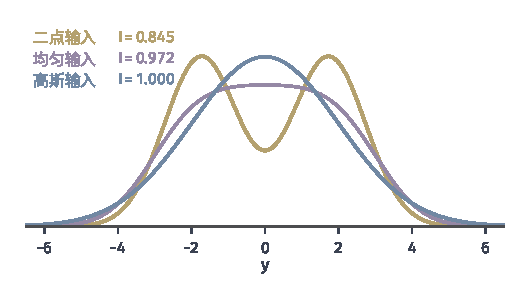
\includegraphics[width=88mm]{figures/07-probability/06-channel-coding/matplotlib/gcc-output-entropy/figure.pdf}
 \caption{$\sigma^2=1$时，三种功率都为$3$的输入经过信道后的输出密度：二点输入$\pm\sqrt3$（黄），$[-3,3]$上的均匀输入（紫），$\mathcal{N}(0,3)$（蓝）。三条输出的方差都是$4$，图中给出对应的互信息（比特）。}
 \label{fig:gcc-output-entropy}
\end{BookInlineFigure}

\subsection{最优输入}
\label{sec:gcc-optimal-input}

上界~\eqref{eq:gcc-upper}的证明中有两处放大：$\operatorname{Var}(Y)\leq P+\sigma^2$，以及固定方差的熵上界。要使两处都取等号，输出必须是方差恰为$P+\sigma^2$的高斯变量。独立高斯变量之和仍是高斯变量（第~\ref{chap:random-variable-transformations}章），所以取$X\sim\mathcal{N}(0,P)$即可：此时$Y\sim\mathcal{N}(0,P+\sigma^2)$。

\begin{theorem}[高斯信道的信息容量]
\label{thm:gcc-capacity}
设$\sigma^2>0$，$P\geq0$。式~\eqref{eq:gcc-info-capacity}中的上确界可以取到，并且
\begin{equation}
 C(P)=\frac12\log_2\Bigl(1+\frac{P}{\sigma^2}\Bigr)\quad\text{比特每次信道使用}.
 \label{eq:gcc-capacity}
\end{equation}
达到最大值的输入分布唯一，是$\mathcal{N}(0,P)$（$P=0$时理解为恒等于零的输入）。
\end{theorem}

\begin{proof}
上界由定理~\ref{thm:gcc-upper}给出。$P>0$时取$X\sim\mathcal{N}(0,P)$与$Z$独立，$Y\sim\mathcal{N}(0,P+\sigma^2)$，由式~\eqref{eq:gcc-mi-entropy}，
\[
 I(X;Y)=\frac12\log_2\bigl(2\pi\mathrm{e}(P+\sigma^2)\bigr)-\frac12\log_2(2\pi\mathrm{e}\sigma^2)=C(P) .
\]
$P=0$时只能$X=0$，$Y=Z$，互信息为零，与公式一致。

再证唯一性，设$P>0$且某个可行输入$X$达到$C(P)$。上界证明中的两处不等式都必须取等号：$Y$的方差等于$P+\sigma^2$，且$Y$是高斯变量。$Y$的方差是$X$的方差加$\sigma^2$，所以
\[
 \operatorname{Var}(X)=P\geq\mathbb{E}[X^2]=(\mathbb{E}X)^2+\operatorname{Var}(X),
\]
于是$\mathbb{E}[X]=0$，$Y\sim\mathcal{N}(0,P+\sigma^2)$。用第~\ref{chap:weak-convergence-of-distributions}章的特征函数，独立和的特征函数是乘积：
\[
 \mathrm{e}^{-(P+\sigma^2)t^2/2}=\phi_Y(t)=\phi_X(t)\,\phi_Z(t)=\phi_X(t)\,\mathrm{e}^{-\sigma^2t^2/2} .
\]
$\phi_Z(t)$处处不为零，两边相除得$\phi_X(t)=\mathrm{e}^{-Pt^2/2}$。特征函数唯一确定分布，所以$X\sim\mathcal{N}(0,P)$。
\end{proof}

比值$P/\sigma^2$称为\term{信噪比}（signal-to-noise ratio，SNR）。容量只依赖信噪比：把输出除以$\sigma$得到噪声方差为$1$、功率为$P/\sigma^2$的信道，接收端可以随时这样做或撤销，传输能力不变。工程上常用分贝表示信噪比，即$10\log_{10}(P/\sigma^2)$。

\paragraph{读容量公式}
公式~\eqref{eq:gcc-capacity}的单位是比特每次实值信道使用。全章的例子$P/\sigma^2=3$给出
\[
 C=\tfrac12\log_2 4=1\ \text{比特每次},
\]
与球的计数一致。把信噪比提到$15$，$1+P/\sigma^2$从$4$变成$16$，容量变成$2$比特：功率增加到五倍，容量只增加一倍。

容量是信噪比的凹函数，图~\ref{fig:gcc-capacity-curve}分两段读它。信噪比很小时，由$\ln(1+u)\leq u$且$u\to0$时二者之比趋于$1$，
\[
 C(P)\leq\frac{\log_2\mathrm{e}}{2}\cdot\frac{P}{\sigma^2},\qquad
 \frac{C(P)}{P/\sigma^2}\to\frac{\log_2\mathrm{e}}{2}\approx0.721\quad(P\to0) .
\]
低信噪比时容量与功率近似成正比，每单位信噪比约值$0.721$比特。信噪比很大时，$\log_2(1+u)-\log_2u\to0$，容量接近$\frac12\log_2(P/\sigma^2)$，功率每增加到四倍（约$6.02$分贝），容量只多$1$比特。

\begin{BookInlineFigure}
 \centering
 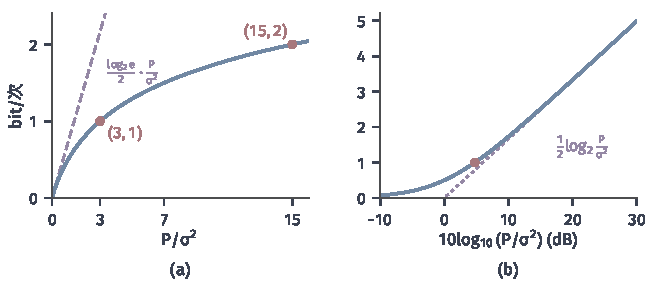
\includegraphics[width=110mm]{figures/07-probability/06-channel-coding/matplotlib/gcc-capacity-curve/figure.pdf}
 \caption{标量高斯信道的容量$C=\frac12\log_2(1+P/\sigma^2)$（蓝）。(a)线性横轴，红点是$(3,1)$和$(15,2)$，紫色虚线是低信噪比时的切线$\frac{\log_2\mathrm{e}}{2}\cdot\frac{P}{\sigma^2}$。(b)横轴为分贝，紫色点线是高信噪比的渐近线$\frac12\log_2(P/\sigma^2)$，斜率约为每$6.02$分贝$1$比特。}
 \label{fig:gcc-capacity-curve}
\end{BookInlineFigure}

\paragraph{有限个输入值的代价}
高斯输入要用到所有实数幅值。若只允许有限个输入值，互信息会低于$C(P)$。等概率二点输入$\pm\sqrt{P}$的互信息不超过$1$比特，无论功率多大；若接收端只记录输出的正负号，信道变成翻转概率$p=\Phi(-\sqrt{P/\sigma^2})$的二元对称信道，速率降为第~\ref{chap:discrete-channel-capacity}章的$1-h_2(p)$，$h_2$是以比特计的二元熵函数。$P/\sigma^2=3$时，$p=0.0416$，三个数是
\[
 C=1.000,\qquad I_{\text{二点}}=0.845,\qquad 1-h_2(p)=0.750 .
\]

图~\ref{fig:gcc-binary-input}把三条曲线画在一起。低信噪比时三者差距很小，因为容量本来就远小于$1$比特，二点输入已经够用；信噪比升高后，二点输入的曲线停在$1$比特，高斯输入继续增长。符号判决丢掉了输出幅值中的可信度信息，由第~\ref{chap:information-measures}章的数据处理不等式，它只能减少互信息。

\begin{BookInlineFigure}
 \centering
 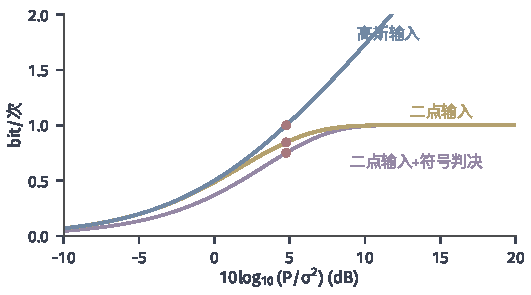
\includegraphics[width=90mm]{figures/07-probability/06-channel-coding/matplotlib/gcc-binary-input/figure.pdf}
 \caption{$\sigma^2=1$时三种传输方式的速率随信噪比（分贝）的变化。蓝：高斯输入，即容量；黄：等概率二点输入，接收端使用实数输出；紫：同样的二点输入，接收端只取输出的正负号。红点对应$P/\sigma^2=3$。}
 \label{fig:gcc-binary-input}
\end{BookInlineFigure}

\paragraph{计量单位}
$C(P)$是每次实值使用的比特数，功率$P$是每次使用的平均能量。改变计量方式时，两者要一起换算。

若每个时刻传送的是一个复数，可以把实部和虚部看成两次实值使用。常见的约定是复噪声的实部与虚部独立，各有方差$\sigma^2/2$，复输入满足$\mathbb{E}\lvert X\rvert^2\leq P$。实部和虚部各分到功率$P/2$时，两次实值使用合计
\[
 2\cdot\frac12\log_2\Bigl(1+\frac{P/2}{\sigma^2/2}\Bigr)=\log_2\Bigl(1+\frac{P}{\sigma^2}\Bigr)\ \text{比特每次复值使用}.
\]
平均分配为什么最优，由第~\ref{sec:gcc-parallel}节的平行信道回答。

若信道每秒使用$m$次，每秒能可靠传送$m\,C(P)$比特，前提是这$m$次使用仍满足本章的模型：噪声独立、方差都是$\sigma^2$，并且$P$指每次使用的功率。若改为给定每秒的总能量，或使用频率改变时噪声方差也随之改变，就要先把这些量折算回每次使用，再代入公式~\eqref{eq:gcc-capacity}。

\subsection{满足功率约束的编码}
\label{sec:gcc-coding}

信息容量是单次使用上的优化值。它是否就是块码的速率极限$C_{\mathrm{op}}(P)$，需要两个方向的证明：低于$C(P)$的速率都可达，高于$C(P)$的速率都不可达。

\begin{theorem}[高斯信道的编码定理]
\label{thm:gcc-coding}
设$\sigma^2>0$，$P>0$。
\begin{enumerate}
 \item 对每个$R<C(P)$，存在一列满足功率约束$P$的$(M_n,n)$码，$M_n\geq2^{nR}$，并且最大错误概率$\lambda_{\max}\to0$。
 \item 任意一列满足功率约束$P$的码，若平均错误概率$P_{\mathrm{e}}\to0$，则$\limsup_{n\to\infty}\frac1n\log_2M_n\leq C(P)$。
\end{enumerate}
因此$C_{\mathrm{op}}(P)=C(P)$；$P=0$时两者都是$0$。
\end{theorem}

\paragraph{为什么不能照搬典型集计数}
第~\ref{chap:discrete-channel-capacity}章的可达性证明数的是典型序列的个数：有限字母表上长为$n$的序列只有有限多个，每个典型序列的概率约为$2^{-nH}$。连续输入下，任何一个具体序列的概率都是零，“个数”没有意义，也不能把$2^{-nH}$中的$H$直接换成可以为负的微分熵。可以保留的是另一样东西：信道条件密度与输出边缘密度之比。下面用它的对数代替典型性。

\paragraph{信息密度}
选一个略低于预算的功率$P'\in(0,P)$，让码字的坐标独立地服从$\mathcal{N}(0,P')$。在这个输入分布下，输出的边缘密度是$g_{P'+\sigma^2}$。

\begin{definition}[信息密度]
\label{def:gcc-info-density}
对输入分布$\mathcal{N}(0,P')$，单次使用的\term{信息密度}（information density）是
\begin{equation}
 i(x;y)=\log_2\frac{g_{\sigma^2}(y-x)}{g_{P'+\sigma^2}(y)} ,
 \label{eq:gcc-info-density}
\end{equation}
长度为$n$的块上的信息密度是逐坐标之和$i_n(x^n;y^n)=\sum_{i=1}^{n}i(x_i;y_i)$。
\end{definition}

$i(x;y)$比较两种解释：$y$是$x$经过噪声得到的，还是与$x$无关地随机出现的。它为正，说明$y$更像由$x$产生。把两个高斯密度代入并展开，
\begin{equation}
 i(x;y)=C(P')+\frac{\log_2\mathrm{e}}{2}\Bigl(\frac{y^2}{P'+\sigma^2}-\frac{(y-x)^2}{\sigma^2}\Bigr) .
 \label{eq:gcc-info-density-explicit}
\end{equation}
信息密度有两个用途，分别对应发送的码字和其余的码字。

第一，对发送的码字及其输出，$i_n$集中在$nC(P')$附近。设$X\sim\mathcal{N}(0,P')$，$Y=X+Z$。此时$Y^2/(P'+\sigma^2)$与$Z^2/\sigma^2$都服从$\chi^2_1$，均值为$1$，所以$\mathbb{E}[i(X;Y)]=C(P')$，这正是式~\eqref{eq:gcc-mi-entropy}的互信息。再算方差：两项的方差都是$2$；$Y$与$Z$是联合高斯的零均值变量，对这样的变量有
\[
 \operatorname{Cov}(Y^2,Z^2)=2\operatorname{Cov}(Y,Z)^2=2\sigma^4 ,
\]
因此
\[
 \operatorname{Var}\Bigl(\frac{Y^2}{P'+\sigma^2}-\frac{Z^2}{\sigma^2}\Bigr)=2+2-\frac{4\sigma^4}{(P'+\sigma^2)\sigma^2}=\frac{4P'}{P'+\sigma^2} .
\]
乘以$(\log_2\mathrm{e}/2)^2$，单次信息密度的方差是
\begin{equation}
 V(P')=\operatorname{Var}\bigl(i(X;Y)\bigr)=(\log_2\mathrm{e})^2\,\frac{P'}{P'+\sigma^2} .
 \label{eq:gcc-info-variance}
\end{equation}
$i_n$是$n$个独立同分布项之和，均值$nC(P')$，方差$nV(P')$。

第二，对与输出无关的码字，$i_n$很少超过高的门限。设$\bar{X}^n$的坐标独立服从$\mathcal{N}(0,P')$，与$Y^n$独立，$Y^n$的坐标独立服从$\mathcal{N}(0,P'+\sigma^2)$。$(\bar{X}^n,Y^n)$的联合密度是乘积$q(x^n,y^n)=f(x^n)\prod_ig_{P'+\sigma^2}(y_i)$，而发送与输出配对时的联合密度是$p(x^n,y^n)=f(x^n)\prod_ig_{\sigma^2}(y_i-x_i)$，$f$是输入块的密度。由定义，二者之比正是
\[
 \frac{q(x^n,y^n)}{p(x^n,y^n)}=2^{-i_n(x^n;y^n)} .
\]
于是对任意$\gamma$，
\begin{equation}
 \mathbb{P}\bigl(i_n(\bar{X}^n;Y^n)>n\gamma\bigr)=\int_{\{i_n>n\gamma\}}2^{-i_n}\,p\leq2^{-n\gamma}\int p=2^{-n\gamma} .
 \label{eq:gcc-change-of-measure}
\end{equation}
这一步把“独立配对”的概率换成“发送配对”的积分，换算因子就是$2^{-i_n}$，在门限以上它不超过$2^{-n\gamma}$。

\paragraph{例：信息密度的两种分布}
取$\sigma^2=1$，$P'=3$。发送配对时$\mathbb{E}[i]=C(3)=1$，$V=(\log_2\mathrm{e})^2\cdot\frac34=1.561$。独立配对时，$\mathbb{E}[(Y-\bar{X})^2]=(P'+\sigma^2)+P'=7$，代入式~\eqref{eq:gcc-info-density-explicit}，
\[
 \mathbb{E}[i(\bar{X};Y)]=1+\frac{\log_2\mathrm{e}}{2}\Bigl(1-7\Bigr)=1-3\log_2\mathrm{e}=-3.33 .
\]
图~\ref{fig:gcc-info-density}画出$n=20$与$n=200$时两种配对的$i_n/n$的直方图。块长增大，两个直方图分别收拢到$1$和$-3.33$；在两者之间放一个门限$\gamma$，发送的码字几乎总在门限之上，独立的码字几乎总在门限之下。

\begin{BookInlineFigure}
 \centering
 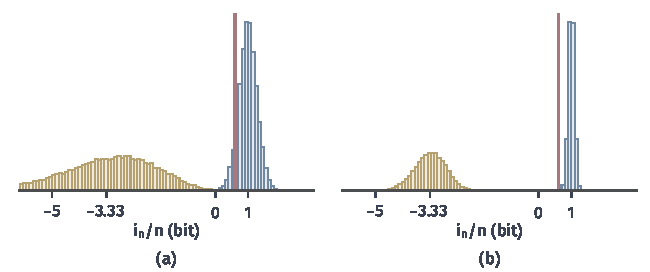
\includegraphics[width=110mm]{figures/07-probability/06-channel-coding/matplotlib/gcc-info-density/figure.pdf}
 \caption{$\sigma^2=1$、码字坐标服从$\mathcal{N}(0,3)$时归一化信息密度$i_n/n$的直方图（种子$7$，每个直方图$20000$对）。蓝：发送的码字与其输出，均值$1$；黄：与输出独立的码字，均值$-3.33$。红线是门限$\gamma=0.6$。(a)$n=20$，蓝色样本有$7.3\%$落在门限以下。(b)$n=200$，没有蓝色样本落在门限以下，也没有黄色样本落在门限以上。}
 \label{fig:gcc-info-density}
\end{BookInlineFigure}

\paragraph{随机码本与阈值判决}
现在构造码。给定$R<C(P)$，由$C$的连续性和严格单调性，可以依次选出
\[
 0<P'<P,\qquad R<\gamma<C(P') .
\]
取$M_n=2^{\lceil nR\rceil+1}$。码本由$M_n$个独立的随机码字$X^n(1),\dots,X^n(M_n)$组成，每个码字的坐标独立服从$\mathcal{N}(0,P')$。解码采用\term{阈值判决}（threshold decoding）：收到$y^n$后，若恰有一个$m$满足$i_n(X^n(m);y^n)>n\gamma$，判为这个$m$；否则判为$1$。

随机码字有可能超过预算，这样的码字不允许发送。分析时采取保守的记账：若$\lVert X^n(m)\rVert_2^2>nP$，就把消息$m$的条件错误概率记为$1$。

\paragraph{例：一次阈值判决}
用一个极小的码本走一遍判决过程。取$\sigma^2=1$，$P'=3$，$n=2$，门限$\gamma=0.6$，即要求$i_2>1.2$。三条码字和收到的输出是
\[
 \begin{gathered}
  x^2(1)=(1.5,-2.0),\quad x^2(2)=(-1.0,1.0),\quad x^2(3)=(2.0,1.5);\\
  y^2=(1.2,-1.4) .
 \end{gathered}
\]
由式~\eqref{eq:gcc-info-density-explicit}，此时
\[
 i(x;y)=1+\frac{\log_2\mathrm{e}}{2}\Bigl(\frac{y^2}{4}-(y-x)^2\Bigr) .
\]
对码字$1$的第一个坐标，$y^2/4=0.36$，$(y-x)^2=0.09$，代入得$1.195$；第二个坐标得$1.094$。三条码字的块信息密度分别是
\[
 i_2(x^2(1);y^2)=2.289,\quad i_2(x^2(2);y^2)=-5.033,\quad i_2(x^2(3);y^2)=-3.915 .
\]
只有码字$1$越过$1.2$，判为消息$1$。码字$3$的第一个坐标与输出也相当接近，信息密度为$0.798$，但第二个坐标相差$2.9$，在噪声标准差为$1$的信道上很不可能，贡献了$-4.713$，整块被否决。块信息密度把各坐标的证据加起来，一个坐标上的偶然吻合抵不过其他坐标上的明显不符。

\paragraph{三类错误}
由对称性，只需分析消息$1$，并对码本的随机性取平均。消息$1$被记为错误，只可能是下面三件事之一发生：
\begin{enumerate}
 \item $E_0$：码字超预算，$\lVert X^n(1)\rVert_2^2>nP$；
 \item $E_1$：发送的码字没有越过门限，$i_n(X^n(1);Y^n)\leq n\gamma$；
 \item $E_2$：某个其他码字越过了门限，即存在$m\neq1$使$i_n(X^n(m);Y^n)>n\gamma$。
\end{enumerate}
三件事都不发生时，恰有消息$1$越过门限，判决正确。三个概率可以分别估计。

$E_0$：$X_i^2$独立同分布，均值$P'$，方差$2P'^2$。由第~\ref{chap:tail-probabilities}章的Chebyshev不等式，
\[
 \mathbb{P}(E_0)=\mathbb{P}\Bigl(\sum_{i=1}^{n}(X_i^2-P')>n(P-P')\Bigr)\leq\frac{2P'^2}{n(P-P')^2} .
\]

$E_1$：$i_n$的均值是$nC(P')$，方差是$nV(P')$，门限$n\gamma$比均值低$n(C(P')-\gamma)$。同样由Chebyshev不等式，
\[
 \mathbb{P}(E_1)\leq\frac{V(P')}{n\bigl(C(P')-\gamma\bigr)^2} .
\]

$E_2$：每个$m\neq1$的码字与发送的码字独立，也与噪声独立，所以与$Y^n$独立，式~\eqref{eq:gcc-change-of-measure}适用。对$M_n-1$个码字用并集界，并利用$M_n\leq2^{nR+2}$，
\[
 \mathbb{P}(E_2)\leq(M_n-1)\,2^{-n\gamma}\leq4\cdot2^{-n(\gamma-R)} .
\]

三项相加，对码本取平均后，消息$1$的记账错误概率不超过
\begin{equation}
 \varepsilon_n=\frac{2P'^2}{n(P-P')^2}+\frac{V(P')}{n\bigl(C(P')-\gamma\bigr)^2}+4\cdot2^{-n(\gamma-R)} ,
 \label{eq:gcc-random-code-bound}
\end{equation}
三项都随$n\to\infty$趋于零。前两项来自大数律，按$1/n$减小；第三项来自门限与码率之间的余量$\gamma-R$，按指数减小。

以$\sigma^2=1$、$P=3$、$R=0.5$为例，取$P'=2.4$，$\gamma=0.7$。此时$C(P')=\frac12\log_2 3.4=0.883$，$V(P')=1.469$。$n=400$时式~\eqref{eq:gcc-random-code-bound}的三项约为
\[
 0.080,\qquad 0.110,\qquad 3\times10^{-24} .
\]
Chebyshev界相当粗：图~\ref{fig:gcc-codeword-energy}的精确计算表明，$n=400$时码字超预算的概率只有$0.00048$，而不是$0.080$。证明只需要这些界趋于零，不需要它们精确。

\begin{BookInlineFigure}
 \centering
 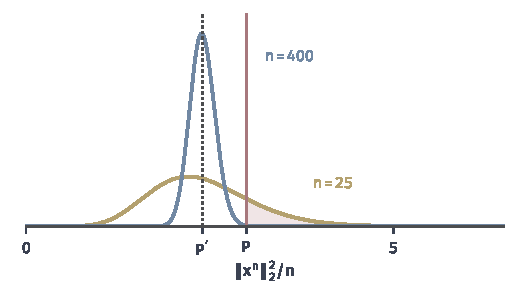
\includegraphics[width=88mm]{figures/07-probability/06-channel-coding/matplotlib/gcc-codeword-energy/figure.pdf}
 \caption{坐标独立服从$\mathcal{N}(0,P')$的随机码字的每坐标能量$\lVert x^n\rVert_2^2/n$的精确密度，$P'=2.4$，预算$P=3$（红线），点线标出$P'$。黄：$n=25$；蓝：$n=400$。红色阴影是超预算的概率，$n=25$时为$0.181$，$n=400$时为$0.00048$。}
 \label{fig:gcc-codeword-energy}
\end{BookInlineFigure}

\paragraph{从随机码本到确定的码}
式~\eqref{eq:gcc-random-code-bound}是对码本取平均的结果。由对称性，每条消息的平均记账错误都相同，所以$\frac1{M_n}\sum_m\tilde{\lambda}_m$对码本的平均也不超过$\varepsilon_n$，其中$\tilde{\lambda}_m$表示消息$m$的记账错误概率。平均值不超过$\varepsilon_n$，至少有一个码本取到不超过$\varepsilon_n$的值；固定这个码本。

这个码本中，记账错误超过$2\varepsilon_n$的消息至多占一半，否则平均值会超过$\varepsilon_n$。删去记账错误最大的一半消息，保留$M_n/2=2^{\lceil nR\rceil}\geq2^{nR}$条，每条都满足$\tilde{\lambda}_m\leq2\varepsilon_n$。当$n$足够大使$2\varepsilon_n<1$时，被保留的码字都不超预算，因为超预算的码字记账错误是$1$。

解码器改为只在保留的码字中做阈值判决。对一条保留的消息，新的错误事件包含在原来的$E_1$与“某个保留的其他码字越过门限”之并中，后者又包含在原来的$E_2$中，所以错误概率不会增加。这样得到的码满足功率约束，码率至少为$R$，最大错误概率不超过$2\varepsilon_n\to0$，定理~\ref{thm:gcc-coding}的第一条得证。

\begin{BookInlineFigure}
 \centering
 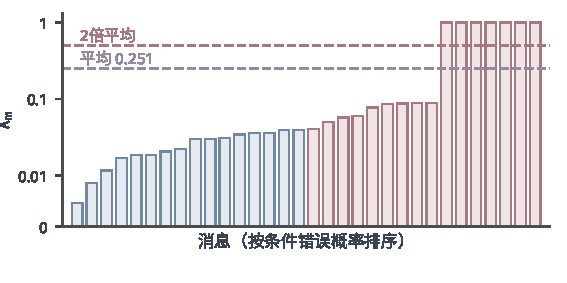
\includegraphics[width=96mm]{figures/07-probability/06-channel-coding/matplotlib/gcc-expurgation/figure.pdf}
 \caption{一个随机高斯码本（种子$5$，$n=12$，$M=32$，$P'=2.4$，$P=3$，$\sigma^2=1$，最近码字判决）中各消息的条件错误概率$\lambda_m$，按大小排序，每条消息用$20000$次噪声模拟估计。超预算的$7$个码字记为$1$。紫色虚线是平均值$0.251$，红色虚线是平均值的两倍；红色柱是删去的一半，保留的消息错误都在$0.04$以下。纵轴在$0.01$以下为线性刻度，以上为对数刻度。}
 \label{fig:gcc-expurgation}
\end{BookInlineFigure}

图~\ref{fig:gcc-expurgation}在一个很短的码上演示这一步。码长只有$12$时，$32$个随机码字中有$7$个超预算，把平均错误抬到$0.251$；删去最差的一半，超预算的码字全部被删掉，剩下的$16$条消息错误都在$0.04$以下。块长增大时，超预算的比例和其他错误都趋于零，删去一半只让码率损失$1/n$。

\paragraph{块长的作用}
证明保证错误趋于零，但没有说多长的块才够。图~\ref{fig:gcc-random-code}用模拟给出一个印象：码率固定为$R=\frac12$，码字取随机方向、长度恰为$\sqrt{nP}$，从而每条码字都恰好用满预算，接收端选与输出最近的码字。$C(P)=\frac12$对应$P/\sigma^2=1$，即$0$分贝。块长从$8$增加到$32$，错误率曲线变陡，在容量对应的信噪比右侧下降得越来越快；但$n=32$时，要把错误率压到$10^{-3}$，信噪比仍需高出约$4$分贝。逼近容量需要长得多的块和高效的译码方法，这是第~\ref{chap:channel-codes}章的话题。

\begin{BookInlineFigure}
 \centering
 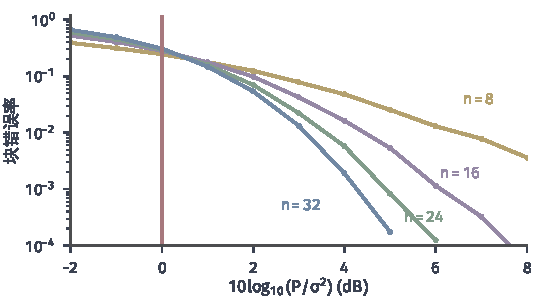
\includegraphics[width=92mm]{figures/07-probability/06-channel-coding/matplotlib/gcc-random-code/figure.pdf}
 \caption{码率$R=\frac12$的随机码在$\sigma^2=1$的高斯信道上的块错误率随信噪比（分贝）的变化，最近码字判决。码字是随机方向上长度为$\sqrt{nP}$的向量。黄、紫、绿、蓝分别对应$n=8,16,24,32$（$M=2^{n/2}$），每点模拟$40000$条消息（种子$11$）。红线是$C(P)=\frac12$对应的$0$分贝。}
 \label{fig:gcc-random-code}
\end{BookInlineFigure}

\paragraph{逆定理}
现在证明第二条：速率超过$C(P)$时，错误不能趋于零。思路与离散信道相同，只是单次互信息的上界换成定理~\ref{thm:gcc-upper}，并且要处理各时刻功率不同的情形。

设$(M,n)$码满足功率约束$P$，消息$W$在$\{1,\dots,M\}$上均匀分布，$X^n=x^n(W)$，$Y^n$是输出。第$i$个时刻在消息上的平均功率记作
\[
 P_i=\mathbb{E}[X_i^2]=\frac1M\sum_{m=1}^{M}x_i(m)^2 .
\]
对$i$求平均，由约束~\eqref{eq:gcc-power}，
\[
 \frac1n\sum_{i=1}^{n}P_i=\frac1M\sum_{m=1}^{M}\frac1n\lVert x^n(m)\rVert_2^2\leq P .
\]

第一步，由第~\ref{chap:information-measures}章的Fano不等式和数据处理不等式，
\[
 \log_2M=H(W)=I(W;Y^n)+H(W\mid Y^n)\leq I(X^n;Y^n)+1+P_{\mathrm{e}}\log_2M .
\]

第二步，上界$I(X^n;Y^n)$。$X^n$只取有限个值，引理~\ref{lem:gcc-output}的证明逐字推广到$n$维：$Y^n$有密度，$h(Y^n)$有限，并且$I(X^n;Y^n)=h(Y^n)-h(Z^n)$。噪声坐标独立，$h(Z^n)=\sum_ih(Z_i)$；由微分熵的链式法则和“条件化不增加熵”，$h(Y^n)\leq\sum_ih(Y_i)$。于是
\[
 I(X^n;Y^n)\leq\sum_{i=1}^{n}\bigl(h(Y_i)-h(Z_i)\bigr)\leq\sum_{i=1}^{n}C(P_i) ,
\]
最后一步对每个时刻用了定理~\ref{thm:gcc-upper}的证明：$\operatorname{Var}(Y_i)\leq P_i+\sigma^2$。

第三步，用凹性合并各时刻。$C(p)=\frac12\log_2(1+p/\sigma^2)$是$p$的凹增函数，由Jensen不等式，
\[
 \sum_{i=1}^{n}C(P_i)\leq n\,C\Bigl(\frac1n\sum_{i=1}^{n}P_i\Bigr)\leq n\,C(P) .
\]
图~\ref{fig:gcc-concavity}说明这一步：把功率在时刻之间不均匀地分配，各时刻上界的平均落在弦上，低于平均功率处的曲线值。

\begin{BookInlineFigure}
 \centering
 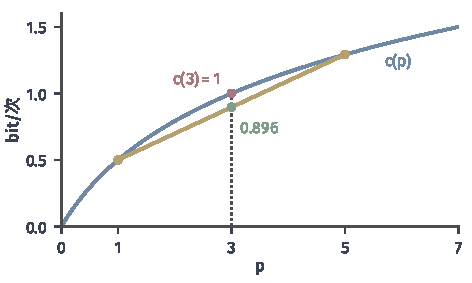
\includegraphics[width=80mm]{figures/07-probability/06-channel-coding/matplotlib/gcc-concavity/figure.pdf}
 \caption{$c(p)=\frac12\log_2(1+p)$（蓝，$\sigma^2=1$）的凹性。一半时刻用功率$1$、一半用$5$，平均功率为$3$；各时刻上界的平均是弦的中点$0.896$（绿），低于$c(3)=1$（红）。}
 \label{fig:gcc-concavity}
\end{BookInlineFigure}

三步合起来，
\begin{equation}
 \log_2M\leq\frac{n\,C(P)+1}{1-P_{\mathrm{e}}} .
 \label{eq:gcc-converse}
\end{equation}
对一列满足约束的码，若$P_{\mathrm{e}}\to0$，两边除以$n$再取上极限，便知码率$\frac1n\log_2M_n$的上极限不超过$C(P)$。定理~\ref{thm:gcc-coding}的第二条得证。

式~\eqref{eq:gcc-converse}也给出错误的下界。以$\sigma^2=1$、$P=3$为例，若码率为$1.2$比特，$\log_2M=1.2n$，整理得
\[
 P_{\mathrm{e}}\geq1-\frac{n+1}{1.2n}\to\frac16 .
\]
块再长，平均错误也不会低于约$16.7\%$。错误概率实际上趋于一，这称为强逆定理，它在这个模型中也成立，但证明需要对信息密度作更细的集中估计，本章不给出证明。

逆定理只用了$\frac1n\sum_iP_i\leq P$，即在消息和时刻上同时平均的功率不超过$P$。所以即使把逐条码字的约束放宽为对消息平均的约束，速率上限仍是$C(P)$；而可达性部分构造的码满足逐条约束。两种约束给出同一个容量。
